% Section content template for individual Educative lessons
% This file contains the actual content for a specific section
% Generated from Educative API section content

% Section: Indexing in a Distributed Search
% Section ID: 6595902341120000
% Section Slug: indexing-in-a-distributed-search
% Generated: 2025-12-07T21:51:34.594939

We'll first describe what indexing is, and then we'll make our way toward distributing indexes over many nodes.\\

\subsection{Indexing}\label{dkjyr_wdUR88EZ2MdpG2q}
\\
\textbf{Indexing} is the organization and manipulation of data that's done to facilitate fast and accurate information retrieval.

\subsubsection{Build a searchable index}\label{C0iN99pn8oBqZWtmTeZb3}
\\
The simplest way to build a searchable index is to assign a unique ID to each document and store it in a database table, as shown in the following table. The first column in the table is the ID of the text and the second column contains the text from each document.

\textbf{Simple Document Index}

\begin{table}[htbp]
\centering
\small
\adjustbox{max width=\textwidth}{
\begin{tabular}{|p{0.475\textwidth}|p{0.475\textwidth}|}
\hline
\textbf{ID} & \textbf{Document Content} \\
\hline
\hline
1 & Elasticsearch is the distributed and analytics engine that is based on REST APIs. \\
\hline
2 & Elasticsearch is a Lucene library-based search engine. \\
\hline
3 & Elasticsearch is a distributed search and analytics engine built on Apache Lucene. \\
\hline
\end{tabular}
}
\caption{Simple Document Index}
\end{table}

The size of the table given above would vary, depending on the number of documents we have and the size of those documents. The table above is just an example, and the content from each document only consists of one or two sentences. With an actual, real-world example, the content of every document in the table could be pages long. This would make our table quite large. Running a search query on the document-level index given above isn't a fast process. On each search request, we have to traverse all the documents and count the occurrence of the search string in each document.
\begin{quote}
\textbf{Note:} For a \textbf{fuzzy search}(This type of search uses approximate string matching rather than exact matching to match the results against the search term.), we also have to perform different pattern-matching queries. Many strings in the documents would somehow match the searched string. First, we must find the unique candidate strings by traversing all of the documents. Then, we must single out the most approximate matched string out of these strings. We also have to find the occurrence of the most matched string in each document. This means that each search query takes a long time.
\end{quote}
\\
The response time to a search query depends on a few factors:

\begin{itemize}
\item
\protect\phantomsection\label{tz7VBQp_TEN5WZXiOcn_n}
The data organization strategy in the database.
\item
\protect\phantomsection\label{jDazfXHjF6GhNZsFtT-hl}
The size of the data.
\item
\protect\phantomsection\label{Ytk3n0Fvl72vX9s7NPQPm}
The processing speed and the RAM of the machine that's used to build the index and process the search query.
\end{itemize}
\\
Running search queries on billions of documents that are document-level indexed will be a slowprocess, which may take many minutes, or even hours. Let 's look at another data organization and processing technique that helps reduce the search time.
\\
\paragraph{Inverted index}\label{h3Ucj57crNYPulaopwc-W}
\\
An \textbf{inverted index} is a HashMap-like data structure that employs a document-term matrix. Instead of storing the complete document as it is, it splits the documents into individual words. After this, the \textbf{document-term matrix}(A document-term matrix is a mathematical matrix that represents the frequency of terms in a list of documents.) identifies unique words and discards frequently occurring words like ``to,'' ``they,'' ``the,'' ``is,'' and so on. Frequently occurring words like those are called \textbf{stop words}. The document-term matrix maintains a \textbf{term-level index} through the identification of unique words and the deletion of unnecessary terms.
\\
For each term, the index computes the following information:

\begin{itemize}
\item
\protect\phantomsection\label{6yERWb2sV_NTaYEmGGuyY}
The list of documents in which the term appeared.
\item
\protect\phantomsection\label{4mMHkwhATYqnCzgV9W_vl}
The frequency with which the term appears in each document.
\item
\protect\phantomsection\label{2s0QNXWGnyGtIEPib3C8K}
The position of the term in each document.
\end{itemize}

\textbf{Inverted Index}

\begin{table}[htbp]
\centering
\small
\adjustbox{max width=\textwidth}{
\begin{tabular}{|p{0.251\textwidth}|p{0.699\textwidth}|}
\hline
\textbf{Term} & \textbf{Mapping} \textbf{( {[} doc{]}, {[} freq{]}, {[}{[} loc{]})} \\
\hline
\hline elasticsearch & ( {[}1, 2, 3{]}, {[}1, 1, 1{]}, {[}{[}1{]}, {[}1{]}, {[}1{]}{]} ) \\
\hline distributed & ( {[}1, 3{]}, {[}1, 1{]}, {[}{[}4{]}, {[}4{]}{]} ) \\
\hline restful & ( {[}1{]}, {[}1{]}, {[}{[}5{]}{]} ) \\
\hline search & ( {[}1, 2, 3{]}, {[}1, 1, 1{]}, {[}{[}6{]}, {[}4{]}, {[}5{]}{]} ) \\
\hline analytics & ( {[}1, 3{]}, {[}1, 1{]}, {[}{[}8{]}, {[}7{]}{]} ) \\
\hline engine & ( {[}1, 2, 3{]}, {[}1, 1, 1{]}, {[}{[}9{]}, {[}5{]}, {[}8{]}{]} ) \\
\hline heart & ( {[}1{]}, {[}1{]}, {[}{[}12{]}{]} ) \\
\hline elastic & ( {[}1{]}, {[}1{]}, {[}{[}15{]}{]} ) \\
\hline stack & ( {[}1{]}, {[}1{]}, {[}{[}16{]}{]} ) \\
\hline lucene & ( {[}2, 3{]}, {[}1, 1{]}, {[}{[}9{]}, {[}12{]}{]} ) \\
\hline library & ( {[}2{]}, {[}1{]}, {[}{[}10{]}{]} ) \\
\hline
Apache & ( {[}3{]}, {[}1{]}, {[}{[}11{]}{]} ) \\
\hline
\end{tabular}
}
\caption{Inverted Index}
\end{table}

In the table above, the ``Term'' column contains all the unique terms that are extracted from all of the documents. Each entry in the ``Mapping'' column consists of three lists:

\begin{itemize}
\item
\protect\phantomsection\label{LqWXv4W7sXJPesw7deD_R}
A list of documents in which the term appeared.
\item
\protect\phantomsection\label{AO0zfdSWZ8nYlyJp7qG3N}
A list that counts the frequency with which the term appears in each document.
\item
\protect\phantomsection\label{rihodmHMTy4alvXWDBx1P}
A two-dimensional list that pinpoints the position of the term in each document. A term can appear multiple times in a single document, which is why a two-dimensional list is used.
\end{itemize}
\begin{quote}
\textbf{Note:} Instead of lists, the mappings could also be in the form of tuples--- such as doc, freq, and loc.
\end{quote}
\\
\textbf{Inverted index} is one of the most popular index mechanisms used in document retrieval. It enables efficient implementation of boolean(Boolean searching is based on a symbolic logic method established by George Boole, an English mathematician. It allows you to limit, broaden, or define your search by combining words and phrases with the words AND, OR, and NOT (also known as Boolean operators). Source: Wikipedia), extended boolean(Extended Boolean search overcomes the disadvantages of the Boolean search. The main disadvantage of the boolean search is that it doesn't incorporate term weights in boolean queries, producing either too small or too big result set. Extended boolean search makes use of partial matching and term weights. It assigns a score to the similarity between queries and documents. This way, a document may be relevant if it matches part of the searched terms and is returned as a result, whereas it was not in the Boolean search. Source: Wikipedia)), proximity(The proximity search finds documents wherein two or more term occurrences that are separately matching are within a certain distance, where distance is the number of intermediate words or characters. Source: Wikipedia)), relevance(Relevance search measures the accuracy of the relationship between the search query and the search results. Source: Wikipedia), and many other types of search algorithms.
\\
\textbf{Advantages of using an inverted index}

\begin{itemize}
\item
\protect\phantomsection\label{uedbksLZhxRRqAAKxPcQ8}
An inverted index facilitates full-text searches(Full-text search draws attention to searching for text within large amounts of electronically recorded text data and delivers results that include some or all of the words in the query. Traditional search, on the other hand, would provide exact matches.).
\item
\protect\phantomsection\label{DHkuEtlHgFUG4pfBnVu1K}
An inverted index reduces the time of counting the occurrence of a word in each document at the run time because we have mappings against each term.
\end{itemize}
\\
\textbf{Disadvantages of using an inverted index}

\begin{itemize}
\item
\protect\phantomsection\label{H3APxMeLM-XlEE32ptri1}
There is storage overhead for maintaining the inverted index along with the actual documents. However, we reduce the search time.
\item
\protect\phantomsection\label{Cuamtulj2i92VnK4X_m4L}
Maintenance costs (processing) on adding, updating, or deleting a document. To add a document, we extract terms from the document. Then , for each extracted term, we either add a new row in the inverted index or update an existing one if that term already has an entry in the inverted index. Similarly
, for deleting a document, we conduct processing to find the entries in the inverted index for the deleted document's terms and update the inverted index accordingly.
\end{itemize}
\\
\paragraph{Searching from an inverted index}\label{L9__8c84xpuGJg3sAHRW1}
\\
Consider a system that has the following mappings when we search for the word ``search engine:''

\begin{table}[htbp]
\centering
\small
\adjustbox{max width=\textwidth}{
\begin{tabular}{|p{0.475\textwidth}|p{0.475\textwidth}|}
\hline
\textbf{Term} & \textbf{Mapping} \\
\hline
\hline search & ( {[}1, 2, 3{]}, {[}1, 1, 1{]}, {[}{[}6{]}, {[}4{]}, {[}5{]}{]} ) \\
\hline engine & ( {[}1, 2, 3{]}, {[}1, 1, 1{]}, {[}{[}9{]}, {[}5{]}, {[}8{]}{]} ) \\
\hline
\end{tabular}
}
\end{table}

Both of these words are found in documents 1, 2, and 3. Both words appear once in each document.\\
\strut \\
The word ``search'' is located at position 6 in document 1, at position 4 in document 2, and position 5 in document 3.\\
\strut \\
The word ``engine'' is located at position 9 in document 1, position 5 in document 2, and position 8 in document 3.\\
\strut \\
A single term can appear in millions of documents. Thus, the list of documents returned against a search query could be very long.\\

\begin{quote}
\textbf{Quiz:}
\textbf{Question 1:} Would this technique work when too many documents are found against a single term?
\textbf{Answer:} It probably wouldn't work to return all the documents that are found.

Instead, we should sort them based on the relevance to the search query.

The top results should be returned to the user, instead of returning all the documents.
\end{quote}

\subsubsection{Factors of index design}\label{uXYV98S-tk8kGFLiaOOvl}
\\
Here are some of the factors that we should keep in mind while designing an index:

\begin{itemize}
\item
\protect\phantomsection\label{oXPsXi8gWquGbqD4JRY5u}
\textbf{Size of the index}: How much computer memory, and RAM, is required to keep the index. We keep the index in the RAM to support the low latency of the search.
\item
\protect\phantomsection\label{LM6NNFua9DKnegVrITESv}
\textbf{Search speed}: How quickly we can find a word from an inverted index.
\item
\protect\phantomsection\label{bTT0XCfs-zB8bsxAyyhOS}
\textbf{Maintenance of the index}: How efficiently the index can be updated if we add or remove a document.
\item
\protect\phantomsection\label{xU9YaqTYPuyj4xPB8zxuL}
\textbf{Fault tolerance}: How critical it is for the service to remain reliable. Coping with index corruption, supporting whether invalid data(The data that makes no sense or doesn't exist can affect the performance of our search when added to the index. We have to detect such data before adding it to the index.) can be treated in isolation, dealing with defective hardware, partitioning, and replication are all issues to consider here.
\item
\protect\phantomsection\label{-tYPLSz6S-Gf6AdmZqDqN}
\textbf{Resilience}: How resilient the system is against someone trying to game the system and guard against search engine optimization (SEO) schemes, since we return only a handful of relevant results against a search.
\end{itemize}
\\
In light of the design factors listed above, let's look at some problems with building an index on a centralized system.

\subsection{Indexing on a centralized system}\label{UHUUVQ6WrYRR4jd1FaITF}
\\
In a \textbf{centralized search system}, all the search system components run on a single node, which is computationally quite capable. The architecture of a centralized search system is shown in the following illustration:

\begin{figure}[htbp]
 \centering
 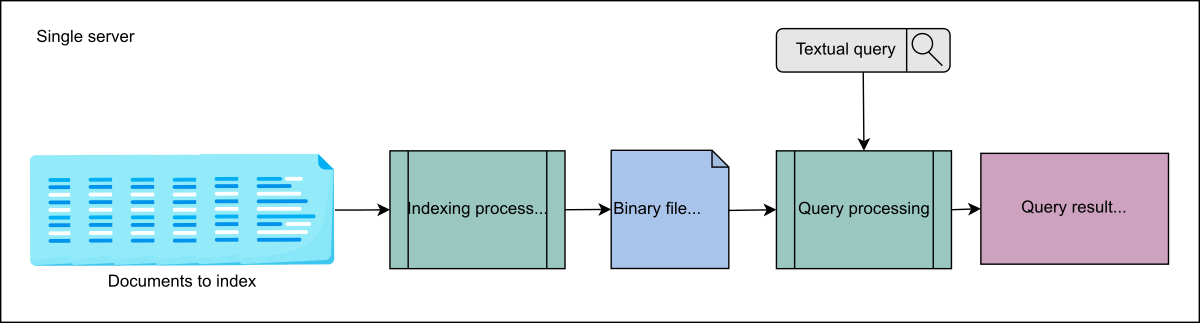
\includegraphics[width=0.5\textwidth]{Images/chapter_21/section_6595902341120000/6545685317287936.png}
 \caption{The architecture of a centralized search system }
\end{figure}

\begin{itemize}
\item
\protect\phantomsection\label{IJyJm67_Jznk1xZB1ya2x}
The \textbf{indexing process} takes the documents as input and converts them into an inverted index, which is stored in the form of a binary file.
\item
\protect\phantomsection\label{-ZJLjImKVqk3hzZVU0HYG}
The \textbf{query processing} or \textbf{search process} interprets the binary file that contains the inverted index. It also computes the intersection of the inverted lists for a given query to return the search results against the query.
\end{itemize}
\\
These are the problems that come with the architecture of a centralized search system:

\begin{itemize}
\item
\protect\phantomsection\label{U-7IMLvL2i37g0MzC0tiA}
SPOF (single point of failure)
\item
\protect\phantomsection\label{ahACln_8vA7mjggkOh049}
Server overload
\item
\protect\phantomsection\label{-5r7AVi4VUMGL2kePgnSK}
Large size of the index
\end{itemize}
\\
\textbf{SPOF}: A centralized system is a single point of failure. If it's dead, no search operation can be performed.
\\
\textbf{Server overload}: If numerous users perform queries and the queries are complicated, it stresses the server (node).
\\
\textbf{Large size of the index}: The size of the inverted index increases with the number of documents, placing resource demands on a single server. The bigger the computer system, the higher the cost and complexity of managing it.
\begin{quote}
\textbf{Note:} With a distributed system, low-cost computer systems are utilized, which is cost effective overall.
\end{quote}
\\
An inverted index needs to be loaded into the main memory when adding a document or running a search query. A large portion of the inverted index must fit into the RAM of the machine for efficiency.
\\
According to \href{https://www.google.com/search/howsearchworks/crawling-indexing/}{Google analytics} in 2022, there are hundreds of billions of web pages, the total size of which is around 100 petabytes. If we make a search system for the worldwide web, the inverted index size will also be in petabytes. This means we have to load petabytes of data into the RAM. It 's impractical and inefficient to increase the resources of a single machine for indexing a billion pages instead of shifting to a distributed system and utilizing the power of parallelization. Running a search query on a single, large inverted index results in a slow response time.
\begin{quote}
\textbf{Note:} Searching a book from a shelf that holds a hundred books is easier than searching a book from a shelf holding a million books. The search time increases with the volume of data we search from.
\end{quote}
\\
Attacks on centralized indexing can have a higher impact than attacks on a distributed indexing system. Furthermore , the odds of bottlenecks (which can arise in server bandwidth or RAM) are also lower in a distributed index.
\\
In this lesson, we learned about indexing, and we looked into the problems of indexing on a centralized system. The next lesson presents a distribution solution for indexing.

% End of section content